\chapter{Economics in \bt}

As mentioned before, \bt~community can be viewed as social networking. Each peer represents a user. A user has \textit{needs}, which is to download a file, to be fulfilled. A file is provided by another user who has different need. This situation creates supply and demand as in traditional economics. This chapter will discuss the economics foundation formed in \bt~system.

As starters, we will discuss the concept of \textit{credit} or \textit{money} in the \bt~system, or in general, in peer-to-peer. The concept of credit is tightly related with the incentive mechanism used in P2P system to maintain the overall performance and to tackle the famous \textit{freeriding problem}. Next, supply and demand condition in \bt~system and its misalignment problem will be elaborated. Another issue which related to credit distribution that leads to system seize-up will be explained afterward. Lastly, the prospecting and investment methodology will be discussed.

The reason why user want to have a lot of credit is motivated by advantages such as higher performance. Individual and community performance must be balanced with each other. \citeauthor{2013:survivepriv:jia} mentioned that oversupply swarm will limit the possibility of giving higher bandwidth allocation for users \cite{2013:survivepriv:jia}. This phenomenon shows that although the intention from user is good, it is not the best case for the swarm perspective. Therefore, it is important for user to choose which community he want to seed to balance those interest. This chapter presents the knowledge needed to observe social-economic phenomenon and to apply suitable policy to improve the overall experience or performance.

%\todo[inline]{invest vs donate. I think we need to stick to just one of them.}

% incentive -> various, centralized, decentralized. Complicated or not. modifying bittorrent protocol? -> not standard 

\section{P2P currency and incentive}
% incentive p2p sveral forms, recipro, reputation, credit
Incentive mechanism in peer-to-peer network is essential as it is one of the property to increase swarm performance. \citeauthor{2011:managesupplydemand:meulpolder} discussed several kinds of incentive mechanism techniques. The technique can be combined and complement each other. Those are : (i) direct reciprocity, (ii) indirect reciprocity, (iii) centralized reputation, (iv) decentralized reputation, and (v) currency \cite{2011:managesupplydemand:meulpolder}. \textit{Reciprocity} focused on the relationship between peers. \bt's \textit{tit-for-tat} is one example. It may be direct between two peers or indirectly by transfer the \textit{trust} to other peer. \textit{Reputation} technique is more straightforward. The information of user behavior in the past is stored (centralized or decentralized). This information iteratively updated and spread through all the peers. BarterCast \cite{2009:bartercast:meulpolder} and MultiChain \cite{2015:multichain:norberhuis} are the example of reputation technique. \textit{Currency}, as we will discuss later, use the concept of \textit{credit}. User need to \textit{buy} the content and can get \textit{credit} by providing service. \textit{Private communities} with SRE is the most common implementation of currency mechanism.

% incentive in p2p example
Different incentive mechanism may be implemented in different type of application. \citeauthor{2015:incentivep2pgame:kang} proposed an incentive mechanism for dynamic and heterogeneous peer with game theory. They take peer capabilities and selfish nature as consideration. The mechanism targeted at wireless and low computing peer which always aim to maximize its own benefit through its credit system. In their system, each peer can set a price for service it provides. The buyer (downloader), in this case, able to negotiate with the seller (uploader) regarding the content price and its bandwidth allocation. This research objective is to maximize the \textit{performance satisfaction factor} where occurred after the transaction \cite{2015:incentivep2pgame:kang}. On the other side, especially in \bt~network, \citeauthor{2010:effortincentive:rahman} proposed effort-based incentive to advocate fairness between peers. They believe that current incentive system disfavor slow peers and eventually will decrease overall performance. In this system, user awarded based on its effort, which is relative on its capacity. This mechanism need alteration in \bt~existing policy on unchoke mechanism and peer selection. However, there is an increasing performance. Download speed for slow peers increase up to 63\% at the expense of decreasing speed for fast peer at 4\%.

% what is credit -> act as a currency
When using currency as the incentive mechanism, it is necessary to define the transaction unit used between the user. In this thesis, we define it as ``credit''. ``Wealth'' is a collection of stored credit on a particular user. Several researches defined credit depend on the case they intend to solve. \citeauthor{2012:economicbt:kash} defined one in his case as \texttt{4 x upload\_bytes - download\_bytes} which is the amount of user can download respecting to DIME share ratio requirement. The credit itself is asymmetrical. From the previous case, for example, if a byte sent from A to B, A will deducted 1 credit, while B will be rewarded by 4 credit \cite{2012:economicbt:kash}. A number of owned credit usually stay linear with another metric called ``reputation'', that is, high credit lead to high reputation as well. Reputation shows how trusted and dependable a user is. 

% terms, content pricing, intro to incentive by example
In his work, \citeauthor{2012:economicbt:kash} defined many economic terms suitable in \bt~community. The \textit{price} of a file is the amount of credit deducted from downloader's wealth. This, in many cases, the same amount uploader will receive and it depend on the size of the file. Commonly, the price per bytes is the same for all the file in the community. However, \citeauthor{2012:economicbt:kash} suggest that a community should carefully declare different price for different files. One way to do it is by lowering the price for the old content, or by defining price depend on the availability and capacity \cite{2012:economicbt:kash}. Often administrator of the private community adopt \textit{freeleech} period which the ``price'' of a file is zero. Therefore, a peer do not need to concern about his credit to download this file \cite{2010:crashsustain:rahman}. However, a user still use his resource to download the files in the \textit{freeleech} period. We argue that in this case, the price is not free, but significantly discounted.


% don't too much / lack of credit
The use of credit in \bt~environment must be implemented with utmost care. \citeauthor{2010:crashsustain:rahman} showed that credit dynamics in P2P community, especially \bt, can lead to system seize-up. There are three statuses observed: \textit{crash}, \textit{crunch}, and \textit{sustain}. Crash and crunch is the condition where there are too much credit and lack of credit, respectively \cite{2010:crashsustain:rahman, 2015:sustainabilitypt:vinko}. To preserve swarm sustainability, there are two aspects that need to be considered. The first one is the swarm condition such as file size and initial credit distribution \cite{2015:sustainabilitypt:vinko}. \citeauthor{2015:sustainabilitypt:vinko} showed that large file size could decrease the sustainability of a swarm. As for initial credit configuration, it depends on the community itself. The wrong amount can crash the system, while with the right amount overall throughput can increase. Secondly, it is the peer behavior \cite{2010:crashsustain:rahman}. \citeauthor{2010:crashsustain:rahman} concluded that selfish peer who only upload in order to continue downloading (freeriding) can badly harm the swarm. Moreover, crash and crunch situation can only be solved with external intervention.

\subsection{Tackling free rider problem}
% what is freeriding and how severe
Incentive mechanism is a straightforward method to counter freeriding and increase cooperation. Freeriding known to reduce the overall performance in peer-to-peer system. In Gnutella, 70\% of its user is not shared any files. Moreover, almost half from total communication only served by 1\% of total peer \cite{2000:freeridegnutella:adar}. If everyone can free ride, the whole system performance may degrade significantly. In other words, freeriding can lead to systematically worse problem called ``tragedy of the commons'' \cite{1968:tragedycommon:hardin}. This problem is popularized by \citet*{1968:tragedycommon:hardin} in \citeyear{1968:tragedycommon:hardin}. This social dilemma emerge because overuse and overexploitation in the shared resource without feedback from the user.

% how can egoist cooperate :  The Emergence of Cooperation among Egoists (Robert Axelrod). Solved by tit-for-tat -> good performance. managing supply and demand meulpowder p.7

% how bittorrent handle freeriding (short term)
\bt~comes with a \textit{tit-for-tat} solution to tackle this issue \cite{2003:bittorrent:cohen}. \textit{Tit-for-tat} in \bt~encourage user to only upload file to one who also has uploaded his file. Furthermore, it is also ranked by upload amount and speed. Freerider always getting low priority in this mechanism. Tit-for-tat valid only in a scope of single torrent. That means, the configuration from one community can not be carried to another community. This causes tit-for-tat works best only in short term transaction and limited parties.

% reputation system (long term)
To complement tit-for-tat mechanism, it is necessary to implement global incentive scheme in \bt. Some researchers start by leveraging the reputation system for peers. This also supported by \citeauthor{2002:reputationtotragedy:milinski} that reputation can help solving ``tragedy of the commons'' problem \cite{2002:reputationtotragedy:milinski}. The mechanism can be centralized on decentralized. Private communities that enforce SRE is an example of centralized mechanism. The reputation of user is stored in the server while it update the data in the communication via tracker. BarterCast \cite{2009:bartercast:meulpolder} and its successor MultiChain \cite{2015:multichain:norberhuis} are the example of decentralized incentive mechanism that works on top of reputation system. 

% freerider behaviour, tit-for-tat result
\citeauthor{2015:freeriderinbtcommunity:das} studied the freerider behavior in \bt~communities. They conclude that freerider in \bt~may not degrade performance as long as the swarm has at least one dedicated and available seeders. The potential availability of seeder also become a factor that keeping the swarm alive. One thing that need to take into consideration is that in their research, they only take four communities as dataset \cite{2015:freeriderinbtcommunity:das}. In \bt, it is unlikely a user will be extremely freeriding, that is not upload anything while keep download data. More common case is the \textit{hit and run} behavior \cite{2011:managesupplydemand:meulpolder}. Hit and run (HnR) is a situation where a user has finished downloading then immediately stop his contribution. Hit and run also often referred as one of the freeriding behavior that peer-to-peer community wanted to prevent.

% cite : The Bittorrent P2P File-Sharing System: Measurements and Analysis

% may include limitation on the effectiveness meulpolder
%Require the change of the system :  \cite{2008:givetogetvod:Mol}. \cite{2010:effortincentive:rahman} \cite{2015:incentivep2pgame:kang}.
% user impossible to be altursitic, not necessary be paranoid. Fairness and system design. While may be reduce performance in spsecific case.

\section{Supply and Demand}
\label{section:suppdemand}
% supply < demand
Supply and demand for both public and private \bt~communities have been studied by \citeauthor{2009:demandsupplyres:andrade} in \citeyear{2009:demandsupplyres:andrade}. \citeauthor{2009:demandsupplyres:andrade} shows that user who contribute more to the community, actually consume a lot from it. This explains that \bt~users are not altruistic enough to seed continuously. Although a significant amount of demand is successfully served by the community, there is only a few swarm that does not suffer from contention. Two hypothetical reasons \citeauthor{2009:demandsupplyres:andrade} suggested are: (i) an asymmetric number of seeder and leecher, which seeder cannot compensate; and (ii) lack of incentive mechanism in the higher level aside from \bt~\textit{tit-for-tat} \cite{2009:demandsupplyres:andrade}. 

% supply in private > in public; flashcrowd increase demand
In public community, there is less supply compared to private community which enforce SRE \cite{2009:demandsupplyres:andrade}. This affects a file longevity because user seed longer in private community. If this behavior happened in long period, it might produce significant imbalance on supply and demand as seeder kept seeding a particular torrent without switching to another swarm. This phenomenon is accumulated by existing of \textit{flashcrowd} effect. Flashcrowd effect is the sudden increase in resource demand due to various reason. Newly published torrent is one of the reasons where flashcrowd effect take place \cite{2013:swarmevolution:su}. These misalignments between supply and demand can worsen the downloading experience in \bt.

% undersupply vs oversupply
In classical file-sharing peer-to-peer system, it is common to see that a swarm is \textit{undersupplied}. Undersupply means that there are not enough resource shared within the swarm to be distributed over the peers who wanted it. The reason why a user join a swarm is to download a file, so that is why undersupplied is commonly occurred. However, with the introduction of private community which enforce upload policy such as SRE or reputation mechanism, the problem shifted to a phenomenon called \textit{oversupply}. Both undersupply and oversupply is the sub-case of supply and demand misalignment. Undersupply condition can be solved by adding more high performance peer to boost download experience. In the other hand, oversupply problem is not trivial to solve.

% oversupply -> fierce upload competition -> unbalance situation
In oversupplied swarm, user may find it difficult to earn the credit by uploading the file. This is because the problem described by \citeauthor{2011:managesupplydemand:meulpolder} called ``upload competition'' \cite{2011:managesupplydemand:meulpolder}. Two conditions from peers perspective must be fulfilled to make P2P system sustain, which is peers must be cooperative, and cooperative peer must stay as long as possible in the swarm \cite{2011:managesupplydemand:meulpolder}. In upload competition problem, cooperative peer can not control his upload rate. The one who will download the seeder chunks is out of the seeder knowledge and control. This may result an expulsion from the community with a SRE because the cooperative peer looks like it do not contribute. \citeauthor{2010:crashsustain:rahman} also stated that oversupply may result to system seize up by \textit{crashing}  \cite{2010:crashsustain:rahman}. Sustainability of a swarm is in a risk in this situation.

% balance -> not sustain
\citeauthor{2011:managesupplydemand:meulpolder} in his work illustrated the relation between various P2P system properties and its relation to system balance. The illustration shown in figure \ref{fig:sysbalance}. Request and seeding behavior is another term of user downloading and uploading behavior, respectively. Seed selection is one part that responsible for choosing which peer to seed. In \cite{2011:managesupplydemand:meulpolder}, \citeauthor{2011:managesupplydemand:meulpolder} showed that using naive random seeding behavior is not sufficient to make P2P system balance. Unbalance system can lead to unsustainable community. Therefore, it is important to work study seeding behavior for each peer by the implementation of credit mining.

\begin{figure}[ht]
	\centering
	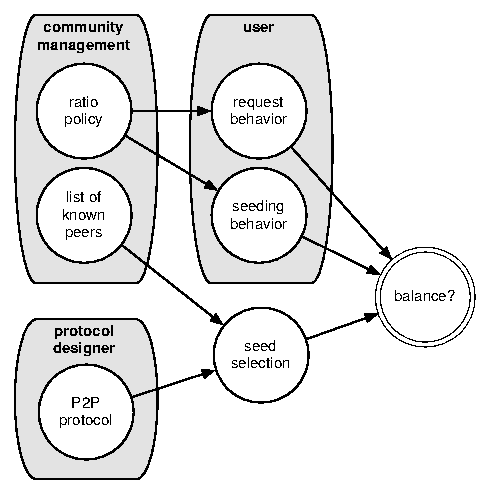
\includegraphics[width=0.7\textwidth]{pics/p2psys_balance.pdf}
	\caption{System properties and its relation to P2P balance \cite{2011:managesupplydemand:meulpolder}.}.
	\label{fig:sysbalance}
\end{figure}


\section{Prospecting and Investment}
% Distinction invest vs donate.
The activity of spending credit can be categorized as three : (i) \textit{trading}, (ii) \textit{investing}, and (iii) \textit{gifting} or \textit{donating}. When a user want to spend his credit to get something, we define it as \textit{trading} or buying. This is most common case, because in credit-based community, every content has its price. \textit{Gifting} is the case when a peer consciously intend to not getting any direct, immediate, or obvious return of his credits \cite{2006:gifting:ripeanu}. The purpose of this action is usually to improve the performance of a community. Gifting can also act as a reward because a peer is satisfied with the community. Investment is the activity of spending credit with the expectation of obtaining credit to use later on. 

% helping others in p2p, improve performance
Recent work on helping other user to increase downloading performance using \bt~ has been done. \citeauthor{2014:cloudseed:leon} uses \bt~ protocol to increase user download speed and at the same time reduce datacenters load. They analyze which swarm or file to help using user bandwidth information and number of connected user\cite{2014:cloudseed:leon}. From another perspective, \citeauthor{2015:coalitionbt:zhang} introduced the \textit{coalition} between \bt~ peers. Coalition is a set of peers that cooperate each other in regards to \bt~policy to minimize download completion time. They also propose coalition-compatible choking strategy to replace the current \bt~one. This research lead to significant performance improvement within the coalition \cite{2015:coalitionbt:zhang}. Although not using \bt~protocol, in \citeyear{2009:p2phelp:he}, \citeauthor{2009:p2phelp:he} proved that helper peer also can improve the streaming capacity in P2P system\cite{2009:p2phelp:he}. \citeauthor{2016:gameauctionp2pstream:mostafavi} extend this work by introducing auction aspect for uploader to choose which user will receive the bandwidth he donate \cite{2016:gameauctionp2pstream:mostafavi}. \citeauthor{2016:gameauctionp2pstream:mostafavi} used game-theory to propose new framework in uncooperative peers with maximizing the credit gain for helpers.

% the importance of healthy swarm -> public good, prevent tragedy of the common. user is selfish, it is good to donate. Reality : they want something in return -> credit. Move the problem into investment problem. 
The ideal situation of balanced high performance and sustainability in \bt~community is desired by align supply and demand as discussed in section \ref{section:suppdemand}. By gifting and helping undersupply community adequately, the ideal situation can be achieved and tragedy of the common can be prevented \cite{2002:reputationtotragedy:milinski}. However, commonly, that is not the case. P2P user are typically selfish in economical way \cite{2014:userbehaviourprivate:jia}. By gifting, it will take ones resource without any return. In fact, common user wanted some return as compensation. Therefore, investment is the most feasible method to balance user and community needs.

% emphasize on investing+prospect
Investing can not be separated by another activity called ``prospecting''. We define \textit{prospecting} as the activity to identify and measure a swarm in the hopes of getting more credit by putting a some credit as capital investment. Prospecting is the initial phase of investment, therefore, it is not needed to be comprehensive and only necessary in smaller scale. In economic perspective, not all undersupplied swarm need to be seeded, even more oversupplied swarm. Choosing a swarm to be seeded is depend on a peer available resource, intention, and investment target. In credit based community, correct investment may spark the community thus improving the performance. From user perspective, good prospecting algorithm can result a high return of the resource used from both investing and prospecting.

% crawl -> part of prospecting, knowing the swarm. 
One important part of prospecting is to identify and measure a particular swarm. Some information can be gathered by querying tracker as central coordinator. A work by \citeauthor{2011:yoshida:crawlbtnet} is the example of contacting tracker regularly to get swarm information \cite{2011:yoshida:crawlbtnet}. As the multi-tracker structure become common, they proposed to contact only one \textit{representative tracker}, which maintain the maximum number of peers in a swarm. BTWorld\footnote{\url{http://btworld.nl/}} has identified four measurement techniques in \bt~\cite{2010:btworld:wojciechowski} as shown in table \ref{tbl:btmeasuremethod}. As investment need real-time data, both \textit{swarm-level} and \textit{peer-level} measurement seems to be the most compatible with prospecting method implementation. Both \textit{internet-level} and \textit{community-level} need compiled data from ISP company and community administrators, respectively \todo{any work how to measure swarm by looking at the peers?}. 

% find low price, sell high price
In classical economic principal, the key to gain benefit is to buy low and sell high. HoweverThis property depends on the item and the market condition. If we translate it into \bt~ economic environment, the item is the file, and the condition is the swarm. \citeauthor{2012:economicbt:kash} introduced term is \textit{resale value}. Resale value is the amount of \textit{gross} credit one will get by uploading a file. In DIME case, it is 4 times uploaded bytes. In other words, resale value is the amount of return one can expect by uploading a file. We saw this mechanism as a way to incentivize user. Because by uploading one byte, a user can get 4 credit which can be used to spend/download 4 bytes. By finding popular item and suitable swarm, the potential of investment become huge.